\section{Überblick der wichtigsten Programmteile} % (fold)
\label{sec:überblick_der_wichtigsten_programmteile}

Im Folgenden wird auf die wichtigsten Teile des Programms nochmal genauer eingegangen und einzelne relevante Algorithmen und Datenstrukturen beschrieben und reflektiert.

\subsection{Model} % (fold)
\label{sub:model}
Das Model teilt sich in drei Hauptkomponenten auf: Die Spielerverwaltung (Leben und Geld) im Paket \class{model.player}, die Levelverwaltung (Zeitlicher Ablauf der Wellen) im Paket \class{model.level} und die Welt an sich im Paket \class{model.maze} mit Kreaturen und Türmen. Das \class{PlayerModelInterface} und die implementierende Klasse \class{Player} sind sehr einfach (eigentlich nur Resourcen erhöhen / verringern) und werden daher nicht genauer betrachtet. Auf die anderen beiden Teile wird dagegen im Folgenden noch genauer eingegangen, wobei die Welt aufgrund der Komplexität noch weiter unterteilt wird. Grundlegend für beide sind Aktionen, die zunächst kurz erklärt werden.

\subsubsection{Akteure und Aktionen} % (fold)
\label{ssub:aktionen}
Alle Objekte, die im Rahmen der Spielzeit agieren, implementieren das \class{ActorInterface} -- ein Funktionales Interface, das nur eine Methode \class{void act(double dt)} beinhaltet. Alle Akteure können beliebig auf das Fortschreiten der GameZeit reagieren. Häufig ist die Entscheidung, was als nächstes getan wird, jedoch nicht bei jedem Tick zu treffen, sondern kann in eine gewisse Spanne andaurnde Aktionen untergliedert werden. Die Klasse \class{Action} bietet eine abstrakte Implementierung eines Akteurs, der solange eine bestimmte Aktion durchführt, bis eine Abbruchbedingung erfüllt ist. Konkrete Implementierungen davon sind \class{CountdownAction}, die als Abbruchbedingung das Ablaufen einer Zeitspanne hat, sowie \class{MoveAction}, die als Abbruchbedingung das Erreichen eines gewissen Punktes oder beweglichen Objektes hat. Diese Klassen bieten die Grundlage für alle wiederholenden Aktionen.
% subsubsection aktionen (end)
\subsubsection{Das Paket \texttt{level}} % (fold)
\label{ssub:level}

Die Aufgabe des Level Pakets ist wie gesagt die zeitliche Steuerung der Creep-Wellen. Sie bietet nach außen für die View ein Binding, wie viel Prozent des Spiels schon vergangen sind. Nach einem gewissen Countdown erstellt sie -- entsprechend der Konfiguration des aktuellen Levels -- eine Liste von Kreaturen in der \class{CreatureFactory} und beauftragt das \class{MazeModelInterface} diese in das Spiel einzufügen. Anschließend wird der Countdown neu gestartet.
% subsubsection level (end)

\missingfigure{Klassendiagramm Level}

\subsubsection{Das Paket \texttt{maze} -- Kreaturen} % (fold)
\label{ssub:maze_kreaturen}
Vieles zu den Kreaturen wurde bereits in den vorherigen Kapiteln (insb \ref{sub:strategy_pattern}) erklärt. Im Folgenden wird sich daher auf die Struktur fokusiert, die bisher noch nicht erwähnt wurde.

Es gibt verschiedene Kreaturenarten, die in einem Enum \class{CreatureType} spezifiziert sind. Dieses Enum enthält auch die Default-Werte der Typen für die Leben, Geschwindigkeit, Wert und Bewegungsalgorithmus. Ausgehend von diesen Default-Werten werden die Creeps in der \class{CreatureFactory} mit einem bestimmten Zeitfaktor abgewandelt (Kreaturen werden mit der Zeit stärker, geben aber auch etwas mehr Geld).

\begin{lstlisting}[language=Java]
public enum CreatureType {
  DUMB(3, 10, 1, new RandomMovement()),
  NORMAL(1, 10, 1, new NoSightMovement()),
  TOUGH(0.8, 30, 3, new NoSightMovement());
  //... Attribute mit Gettern
  private CreatureType(double defaultVelocity, int defaultLifes,
   int defaultValue, MovementInterface defaultMovement) {
   //... Zuweisung
  }
}
\end{lstlisting}

Die Kreaturen sind Akteure und werden daher von der GameLoop aktualisiert. Sie besitzen eine aktuelle \class{Action}, die z.B. eine \class{MoveAction} zu einem bestimmten Ziel ist. Ist dieses Ziel erreicht, sucht die Kreatur mit dem gesetzten Bewegungsalgorithmus das nächste Ziel und erstellt dafür eine neue MoveAction. Zusätzlich wird bei jeder Positionsänderung überprüft, ob Kreaturen in der Reichweite sind, die andere Informationen über die Welt haben (\class{VisitedMap}). Falls das der Fall ist, wird die Bewegungsaktion durch eine \class{CountdownAction} vorübergehend unterbrechen, um sich mit der anderen Kreatur zu unterhalten. Danach wird die Bewegung fortgesetzt.

\paragraph{VisitedMap} Wie bereits in Kapitel~\ref{sub:neuer_ansatz_im_eigenen_projekt} erwähnt, ist die VisitedMap zentraler Bestandteil der scheinbaren Intelligenz der Kreaturen. Da diese sehr oft verglichen wird, war hier eine effiziente Implementierung notwendig. Die Speicherkomplexität der Map liegt in \(O (c\cdot n \cdot m)\), wobei \(c\) die Anzahl der Creeps, und \(n\times m\) die Abmessung der Welt ist (im aktuellen Spiel \(10\times20\)). Sind jedoch alle \(c\) Kreaturen nah zusammen, versucht jede Kreatur mit jeder anderen zu kommunizieren, also \(c\cdot (c-1)\) und jeder Vergleich der Arrays benötigt \(O(n\cdot m)\) Schritte \(\Rightarrow O(c^2\cdot n\cdot m)\). Eine Optimierung gelingt dadurch, dass für die Arrays ein Hash-Wert erstellt wird und für den Vergleich herangezogen wird. Nur wenn die Hash-Werte unterschiedlich sind, wird über das gesamte zweidimensionale Array iteriert und die Informationen zusammengefügt. Dadurch muss in dem gleichen Fall nur eine Kreatur mit allen anderen den Zustand synchronisieren -- alle anderen Vergleiche sind unabhängig von der Spielfeldgröße \(\Rightarrow O(c\cdot n \cdot m + (c-1)\cdot(c-1)\cdot1) = O(c \cdot n \cdot m + c^2) \). Da sich die Figuren in der Regel eine längere Zeit in der Gruppe bewegen, unterscheidet sich der State auch seltener, wodurch der Vorteil des Hashwertes noch deutlich wird. Nicht beachtet wurde dabei bisher die Komplexität zur Berechnung des Hash-Wertes. Zunächst wurde die Methode \class{Arrays.deepHashCode(Object[] a)} zur Berechnung verwendet, die allerdings in Benchmarks immer noch eine hohe Auslastung anzeigte. Stattdessen wurde anschließend das Zobrist Hashing \todo{Referenz} verwendet (genaueres siehe nächster Abschnitt). Das ermöglichte, den Hash-Wert bei Änderungen direkt mit einer einfachen Bit-Operation anzupassen, statt ihn mit dem gesamten Array neu zu berechnen. Dies führte zu einem vernachlässigbaren Aufwand zur Hashberechnung und der Vergleich war effizient genug, dass dies kein Problem mehr darstellte. Die tatsächlich gemessenen Laufzeitergebnisse sind in Abbildung~\ref{fig:benchmark} dargestellt.
\begin{figure}[tb]
	\centering
	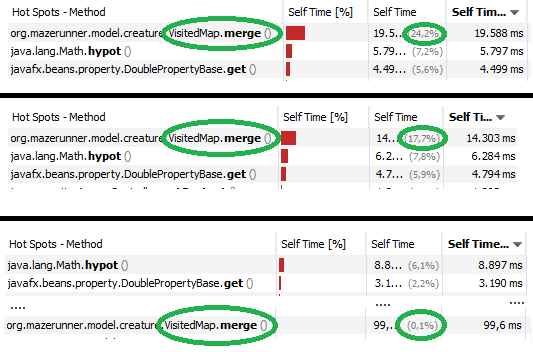
\includegraphics{images/benchmark.png}
	\caption{Laufzeitanalyse der drei Implementierungen der Merge-Methode. Die Daten wurden mit Java Visual VM aufgenommen und zeigen einen Ausschnitt der rechenintensivsten Methoden gemessen zur Laufzeit mit 600 Kreaturen und dem gleichen Labyrinth Setup. Die erste Tabelle zeigt die Laufzeit ohne Hashing, die zweite mit \lstinline{Arrays.deepHashCode}, die dritte die letztliche Programmierung mit Zobrist Hashing.}
	\label{fig:benchmark}
\end{figure}

\subparagraph{Ablauf des Zobrist Hashing} % (fold)
 \label{subp:ablauf_des_zobrist_hashing}
 Beim Zobrist Hashing werden einmalig für jedes Feld in jedem möglichen Zustand ein Bitmuster (in Form eines zufälligen Integers) erzeugt.
\begin{lstlisting}
public class VisitedMap {
  private static int[][][] bitStrings;
  public enum VisitedState { UNKNOWN, VISITED, WALL }

  private void initializeBitStrings(int maxX, int maxY) {
    if (bitStrings == null) {
      bitStrings = new int[maxX][maxY][VisitedState.values().length];
      for (int x = 0; x < maxX; x++) {
        for (int y = 0; y < maxY; y++) {
          for (int j = 0; j < VisitedState.values().length; j++) {
            bitStrings[x][y][j] = new Random().nextInt();
          }
        }
      }
    }
  }
  /* ... */
}
\end{lstlisting}
Der Hash wird dann pro \class{VisitedMap} Objekt (also pro Kreatur) einmal gebildet, indem ausgehend von dem Hash 0 für jedes Feld der VisitedMap das entsprechende Bitmuster mit \emph{XOR} mit dem Hash verknüpft wird. 
\begin{lstlisting}
  private VisitedState[][] map;
  private int hash = 0;

  public VisitedMap(int maxX, int maxY) {
    initializeBitStrings(maxX, maxY);
    map = new VisitedState[maxX][maxY];
    for (int x = 0; x < map.length; x++) {
      for (int y = 0; y < map[x].length; y++) {
        map[x][y] = VisitedState.UNKNOWN;
        hash ^= bitStrings[x][y][VisitedState.UNKNOWN.ordinal()];
      }
    }
  }
\end{lstlisting}
Änderungen können dann einfach vorgenommen werden, indem zuerst mit \emph{XOR} der alte Wert aus dem Hash rausgenommen wird (denn \emph{XOR} ist seine eigene Umkehrfunktion) und der neue Wert mit \emph{XOR} hinzugefügt wird.
\begin{lstlisting}
private void setNewStateOnPosition(int x, int y, VisitedState newState) {
  VisitedState old = map[x][y];
  hash ^= bitStrings[x][y][old.ordinal()] ^ bitStrings[x][y][newState.ordinal()];
  map[x][y] = newState;
}
\end{lstlisting}
 % subparagraph ablauf_des_zobrist_hashing (end)

\paragraph{Wegsuche} Von der konkreten Algorithmik interessant ist bei der Pfadfindung nur die Klasse \class{NoSightMovement}. Das Vorgehen wurde schon in Kapitel~\ref{sub:strategy_pattern} kurz beschrieben. Die Aufgabe des Algorithmus ist es, aus der aktuellen \class{VisitedMap} und der aktuellen Position ein nächstes Ziel zu bestimmen. In Betracht gezogen wurden dafür alle noch unbekannten Felder, also ist das naheste, unbekannte Feld gesucht. Die einfachste Implementierung war, eine Breitensuche wie im Dijkstra-Algorithmus zu beginnen und bei dem ersten unbekannten Feld abzubrechen. Da diese Berechnung nicht in jedem Tick ausgeführt wird, sondern nur wenn eine neue Aktion berechnet wird (bei den normalen Kreaturen also einmal pro Sekunde), ist die Performanz hiervon auch kein Problem gewesen. Tatsächlich ist eine Verbesserung hier gar nicht so leicht: Überlegt war zum Beispiel, ob der Algorithmus beschleunigt werden kann, indem für das gesamte Labyrinth einmalig z.B. mit dem Floyd-Warshall-Algorithmus von allen Punkten aus der kürzeste Weg zu allen anderen Punkten berechnet wird. Statt für jede Aktion den Dijkstra-Algorithmus erneut auszuführen, müsste so nur bei einer Änderung des Labyrinths neuberechnet werden. Das Problem ist allerdings, dass den Kreaturen diese Tabelle nicht so viel nützt, weil sie ihr Ziel nicht kennen, sondern anhand der bereits bekannten Felder ein weiteres suchen wollen. Ebenso ist die Suche mit Dijkstra für diese Aufgabe sehr gut geeignet. Eine algorithmische Verbesserung in diesem Bereich schien also bisher nicht notwendig und konnte von mir auch noch nicht gefunden werden.

\paragraph{Datenstruktur der Kreaturen} Ein Bereich, der im Rahmen des Projektes noch nicht optimiert wurde, ist die Datenstruktur der Kreaturen. Diese sind in einer \class{ObservableList} gespeichert, was der View erlaubt einen \class{ChangeListener} darauf zu registrieren. Die Datenstruktur wurde verwendet, da die Implementierung am einfachsten war, jedoch ist sie ein Engpass für die Berechnungen im Model und aktuell der langsamste Teil im Projekt. Grund dafür ist, dass besonders häufig Bereichsanfragen auf die Kreaturen gestellt werden, beispielsweise wenn ein Tower zum Schießen bereit ist, oder wenn Kreaturen miteinander Kommunizieren wollen. Dementsprechend wäre wahrscheinlich eine Speicherung in einem k-d Baum oder R-Baum effizienter. Das Problem daran ist, dass die Kreaturen sich sehr viel bewegen und somit entweder häufig die aufwändigen Update-Operationen auf den Bäumen ausgeführt werden müssen, oder die Bäume zu jedem Tick mit Bulkload neu erstellt werden müssen. Das stellt einen hohen Anspruch an die Effizienz der Bäume dar.
% subsubsection maze_kreaturen (end)

\subsubsection{Das Paket \texttt{maze}: Türme} % (fold)
\label{ssub:maze_türme}

Grundbausteine zum bilden des Labyrinths sind zunächst Mauern. Diese haben sehr geringe kosten und blockieren die Creeps. Jede Mauer hat eine \class{ObjectProperty} vom generischen Typ \class{AbstractTower}, kann also durch Polymorphie ein beliebiges Objekt der Unterklassen von \class{AbstractTower} besitzen. Diese Unterklassen sind die konkreten Türme, die eigene Upgrades definieren und eine Methode \class{void shoot()} implementieren müssen.

Um ständige \class{null} Überprüfungen zu vermeiden, wurde auch eine Unterklasse \class{NoTower} implementiert, die keinerlei Aktivität übernimmt. Die weiteren Turmarten sind:
\begin{itemize}
  \item \class{NormalTower}: Ein Turm, der nur einmal pro Sekunde schießt, dafür aber relativ stark ist und der billigste Turm ist. Upgrades erhöhen vor allem die Stärke und Reichweite des Turms. Dieser Turm ist die Orientierung für die Stärke der anderen Türme.
  \item \class{FastTower}: Schießt schneller, aber schwächer und kostet etwas mehr. Upgrades sind dafür billiger und verstärken vor allem die Geschwindigkeit und Stärke.
  \item \class{SlowdownTower}: Macht keinen Schaden, sondern verlangsamt die getroffene Kreatur. Schießt selbst langsamer und kostet etwas mehr. Upgrades erhöhen die Geschwindigkeit und verstärken den Slowdown-Effekt.
  \item \class{AmnesiaTower}: Macht keinen Schaden, sondern \enquote{verwirrt} die getroffene Kreatur, indem eine Zeit lang die Wegfindung der Kreatur durch eine zufällige Wegwahl ersetzt wird. Der Turm versucht beim schießen Kreaturen zu finden, die er bisher noch nicht getroffen hat und kann so eine größere Menge an vorbeilaufenden Kreaturen treffen. Es ist der teuerste Turm, jedoch existieren keine Upgrades.
\end{itemize}

Der normale Turm ist auch die Orientierung für Game Balancing Überlegungen wie \zitat{Wie oft muss ein Turm eine normale Kreatur treffen?}, und \zitat{Wie viele Schüsse kann ein Turm auf eine vorbeilaufende Kreatur abgeben?}, nach denen sich die Leben der Kreaturen richten. Die Werte aller anderen Türme werden ebenfalls an den Daten des normalen Turms orientiert festgelegt. Eine automatisierte Anpassung basierend auf Nutzerdaten wurde nicht implementiert, wäre aber grundsätzlich möglich und eine interessante Erweiterung. 

Die Implementierung der Türme verwendet eine \class{CountdownAction}, die das Schießen nach dem entsprechenden Intervall triggert. Da wird zunächst mit einer Bereichsanfragen auf die Kreaturen ein Ziel ausgewählt. Anschließend wird eine Kugel erzeugt, die sich wiederum mit einer \class{MoveAction} zunächst zum Ziel bewegen muss, bevor sie ihre Wirkung entfaltet. Vor allem Letzteres ist wichtig, um den Effekt der Kugel bis zum tatsächlichen Treffen verzögern zu können und nicht direkt in der Schießen-Methode auszuführen. Dadurch ist der Ablauf für den User besser sichtbar und nachvollziehbar.

\missingfigure{UML Klassendiagramm von Tower package}

\paragraph{Datenstruktur der Mauern} Die Datenstruktur im \class{Maze}, die die Mauern hält, ist wie bei den Kreaturen eine \class{ObservableList}. Dadurch kann die View wieder einen Listener auf die Änderungen registrieren. Da die Kreaturen oft anfragen müssen, ob auf einem Feld eine Mauer den Weg blockiert, wurde zusätzlich noch ein zweidimensionales Boolean-Array gespeichert, das allerdings nur intern verwendet wird. Der zusätzliche Speicheraufwand ist zu vernachlässigen, da nur ein einzelnes Maze existiert und somit nur ein Boolean-Array in der Größe des Spielfeldes gespeichert wird. Die Anfragezeit, ob ein Feld belegt ist, konnte dagegen dadurch auf konstante Zeit \(O(1)\) im Gegensatz zu linearer Zeit \(O(w)\) (\(w\) Anzahl der \class{Wall} Objekte) reduziert werden. 

% subsubsection maze_türme (end)
% subsection model (end)
% section überblick_der_wichtigsten_programmteile (end)